%vis at løsningerne findes i hjørnene af en polytop, der er også lidt rod med den danske oversættelse af vertex, som egentligt betyder hjørne måske er der en fagterm???
Som det fremgår i ovenstående, vil en optimal løsning være i hjørnerne af en polyede.
Der er derfor behov for måder at definere disse hjørner på.

\begin{defn}{}{ekstrema}
Lad $P$ være en polyede. en vektor $\mathbf{x} \in P$ kaldes et \textbf{ekstremumspunkt} i $P$, hvis der ikke eksisterer to vektorer $\mathbf{y},\mathbf{z} \in P$ $\mathbf{y} \land \mathbf{z} \neq \mathbf{x}$ samt en skalar $\lambda \in [0,1]$ hvorom det gælder: $\mathbf{x}=\lambda\mathbf{y}+(1-\lambda)z$.
\end{defn}
Et hjørne kan beskrives ud fra denne definition idet der såfremt $\mathbf{x}=\lambda\mathbf{y}+(1-\lambda)z$, og alle vektorene findes i $P$, gælder at $\mathbf{x}$ er en konveks kombination af $\mathbf{y}$ og $\mathbf{z}$.
Hvis $\mathbf{x}=\lambda\mathbf{y}+(1-\lambda)z$ $\mathbf{y}\notin P$ og $\mathbf{x}$ er et ekstremumspunkt må derfor gælde at $\mathbf{y}\notin P$ $\mathbf{z}\notin P$ eller $\mathbf{x}=\mathbf{z}$ eller $\mathbf{x}=\mathbf{y}$. 
Det skal her nævnes at denne definition er strengt geometrisk.


\begin{figure}[h!]
  \centering
  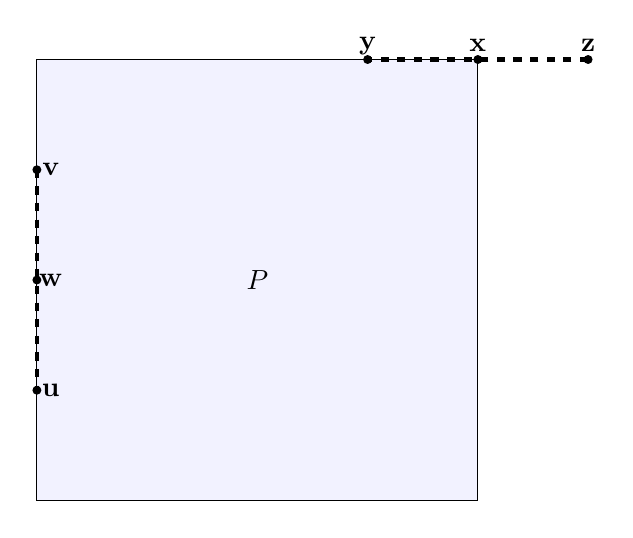
\begin{tikzpicture}[scale=0.7]
    \tikzset{punkt/.style={point, draw=black}}
    
    
%Punkter

	\node at (4,4)	(1){};
	\node at (-4,4)	(4){};
	\node at (4,-4)	(2){};
	\node at (-4,-4) (3){};


	\filldraw[black, fill=blue!5] (2) rectangle (4);
	\node at (0,0) (P){$P$};
	
	\filldraw [black] (2,4) circle (2pt);
	\filldraw [black] (4,4) circle (2pt);
	\filldraw [black] (6,4) circle (2pt);
	\filldraw [black] (-4,2) circle (2pt);
	\filldraw [black] (-4,0) circle (2pt);
	\filldraw [black] (-4,-2) circle (2pt);	
	\node at (2,4.25)	 (y){$\textbf{y}$};
	\node at (4,4.25)	 (x){$\textbf{x}$};
	\node at (6,4.25)	 (z){$\textbf{z}$};
	\node at (-3.75,2)  (v){$\textbf{v}$};
	\node at (-3.75,0)	 (w){$\textbf{w}$};
	\node at (-3.75,-2) (u){$\textbf{u}$};


	\draw[-, dashed,black,ultra thick] (6,4) -- (2,4);
	\draw[-, dashed,black,ultra thick] (-4,2) -- (-4,-2);

  \end{tikzpicture}
  \caption{En afgrænset polytop $P$ hvor $\textbf{x}$ er et ekstramapunkt da der ikke findes vektorer $\textbf{y}$ og $\textbf{z}$ sådan at $\mathbf{x}=\lambda\mathbf{y}+(1-\lambda)z$. $\textbf{w}$ er i modsætning ikke et ekstremapunkt da der findes $\textbf{v}$ og $\textbf{u}$ sådan at $\mathbf{w}=\lambda\mathbf{v}+(1-\lambda)u$.}
  \label{fig:ekstrema}
\end{figure}
%
%
%    \node[punkt] at (-4,0.5)      (v1){$v_1$};
%    \node[punkt] at (-2,0.5)      (v2){$v_2$};
%    \node[punkt] at (-4,-1.5)     (v3){$v_3$};
%    \node[punkt] at (-2,-1.5)     (v4){$v_4$};
%    \node at (-3,2)     (v){$K_{4}$};
%
%
%    \node[punkt] at (4.6,-0.2)      (k1){$v_3$};
%    \node[punkt] at (1.4,-0.2)      (k2){$v_2$};
%    \node[punkt] at (2,-2)     (k3){$v_4$};
%    \node[punkt] at (4,-2)     (k4){$v_5$};
%    \node[punkt] at (3,1)      (k5){$v_1$};
%    \node at (3,2)      (k){$K_{5}$};
%
%
%
%
%
%    \draw [-, thick, draw=black] (v1) -- (v2);
%    \draw [-, thick, draw=black] (v1) -- (v3);
%    \draw [-, thick, draw=black] (v1) -- (v4);
%    \draw [-, thick, draw=black] (v2) -- (v3);
%    \draw [-, thick, draw=black] (v2) -- (v4);
%    \draw [-, thick, draw=black] (v3) -- (v4);

En alternativ geometrisk defintion relatere sig til \textit{hjørner}, som er den entydige optimale løsning til et givet lineært programeringsproblem med den mulige løsningsmængde $P$.
\begin{defn}{}{hjoerner}
Lad $P$ være en polyede. En vektor $\mathbf{x}\in P$ siges at være et \textbf{hjørne} hvis der esksiterer en vektor $\mathbf{c}$ hvorom det gælder at $\mathbf{c}^T\mathbf{x}<\mathbf{c}^T\mathbf{y}$ for alle $\mathbf{y}$ som opfylder $\mathbf{y} \in P$ samt $\mathbf{y}\neq\mathbf{x}$.
\end{defn}
Dette kan ligeledes beskrives som at $\mathbf{x}$ er et hjørne i $P$ såfremt $P$ er på den ene side af et hyperplan der skærer $P$ i $\mathbf{x}$. Jævnfør definitionen har dette hyperplan ligningen $y \mid \mathbf{c}^T\mathbf{x}=\mathbf{c}^T\mathbf{y}$